\chapter{Interactive Musical Score}

\section{Introduction}

Reading music from the score is essential to Western classical music training. Traditionally, children learn the different musical notes by singing or playing notes on an instrument guided by a teacher. We envision a way for children to learn the correspondence between notation and sound by directly touching the score.
The Interactive Score is effortless and allows children to make discoveries independently. The correspondence between the visual, the tactile, and the sound can aid in learning.

In this work, we introduce the Interactive Score, a novel instrumental device for children's solfege learning. Paper scores lay onto a staff drawn with conductive ink and connected to an Adafruit musical box. Pressing a note in the score triggers its sound, and running fingers over the notes play a melody.

% \subsection*{Motivation}

\section{Related work}

\subsection{Context}

A review of music theory pedagogy over the past decade reveals many criticisms about music theory courses. Other concerns include taking a harmonic, melodic, or compositional approach to teaching theory. The early involvement of students in creative thinking about harmony, melody, and rhythm partially determines their success in the academic program \cite{bland1977college}. Developing a feeling for the mastery of the preliminaries to music and the presentation of the basics are the prerequisites for a successful future theoretical education.

However, out of the large number of students who embark on learning music, only a few retain the courage and motivation to continue their studies to the end.
For example, out of 100 French people aged 15 and over, a study recorded that only 30\% of the musicians who have learned music continue practicing their instrument during their lives \cite{amateurs}.

It is pointless and frustrating for students to be pushed too quickly into advanced and sophisticated theory without musically visualizing what they are studying.

\subsection{Approaches}

Music theory courses can take many forms. There are many approaches to developing musicianship skills. Teachers often choose between traditional or more contemporary approaches.

\paragraph*{Traditional approach}

Traditional music lessons prepare students to read, write and perform music from the work of great academic composers. It produces excellent results in terms of sight-reading skills. However, many students leave these music studies because they need more enjoyment of the method.


\paragraph*{Contemporary approach}
Contemporary music lessons are paired with instrumental lessons (usually piano or guitar). They do not require music reading or theory. These lessons focus on skill, musicality, and more intuitive learning methods. They require the student to have a good ear for music and a sense of rhythm. The contemporary approach benefits students with difficulty visualizing with theory classes. They can play real pieces only a few months after starting their lessons. 


The primary advice if a student has any problem understanding music theory is to study with a piano. Intervals and harmonies are easier to understand on a piano first, as is all the rest of the theory.

\subsection{Musical Mental Projection}

Musical imagery, or the ability to create an image of sound in our minds, is an essential
skill for all musicians. For example, brass, winds, strings, and singers imagine the
pitch of an upcoming note to make it easier to play it and determine the distance from
the previous note
\cite{zatorre2005mental}. Composers and arrangers also use musical imagery when creating a new piece. Musical imagery training improves the ability to follow the upward and downward movements of the tonal contour of a musical phrase or imagined tune \cite{weber1986musical}.

Ear training" (or solfege) has traditionally been part of the curriculum of most music
schools. An essential part of solfege is the ability to read music notation and imagine
how it is supposed to sound. We are interested in teaching this skill to children.

\subsection{Tangible Interactive Media for Music Practise}

Many projects aim at getting a child involved in the world of music. However, only some consist of tangible interactive media for music discovery.

For example, Zigelbaum et al. investigated how electronic instruments can engage young learners in learning to make music. Their project was the development of different tools involving movement, linking it to a sound. They created a trampoline, an interactive matrix, or musical bracelets \cite{zigelbaum2006bodybeats}.

Xiao Xiao et Al. propose an understanding of the essential workings of music without going into the details of music theory \cite{xiao2014andante}.
The authors expose a new technique for visualizing musical motion on a piano keyboard. The technique, called Andante, uses walking figures that move along the keyboard to represent the movement of musical phrases. The results of their user test showed that the participants found the Andante animation to be significantly more informative and engaging than the video without animation.

\begin{marginfigure}
   \centering
   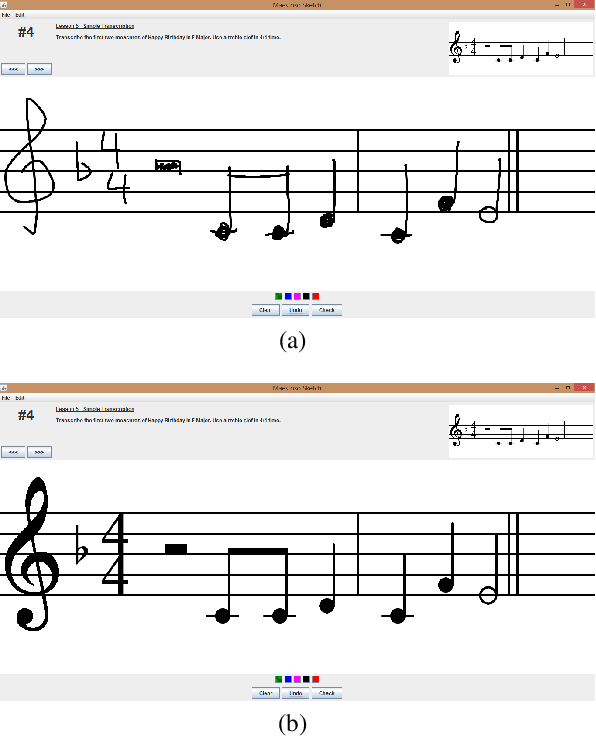
\includegraphics{images/maestoso.png}
   \caption{Maestoso Educational
   Sketching Tool for Learning Music Theory}
   \label{fig:taele2015maestoso}
\end{marginfigure}

The work of Taele et al. \cite{taele2015maestoso} \ref{fig:taele2015maestoso} describes the practical and cognitive benefits of learning music theory for both musicians and non-musicians. The paper proposes an intelligent educational tool to help students learn music theory. The tool, called Maestoso, utilizes sketch-based interaction and machine-learning techniques to provide personalized feedback to the user.
The paper first introduces the importance of music education and the challenges students face when learning music theory, such as the abstract nature of music concepts and the difficulty of translating musical ideas into notation.
Maestoso is a sketching interface that allows users to draw musical notes, chords, and melodies using a stylus or finger. The program uses machine learning algorithms to recognize the user's sketches and provide feedback on their accuracy and completeness.

\begin{marginfigure}
   \centering
   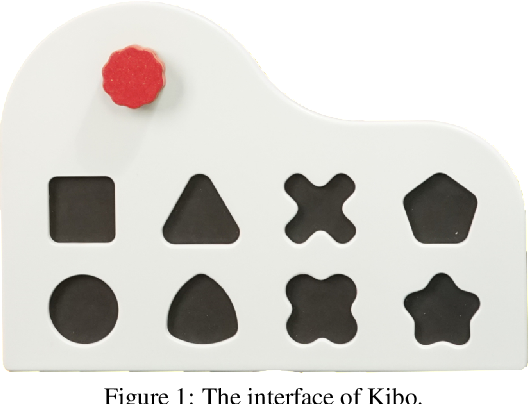
\includegraphics{images/IS_kibo.png}
   \caption{The interface of Kibo}
   \label{fig:amico2020kibo}
\end{marginfigure}

Amico et al. discuss the development of a new type of MIDI controller designed for music education \cite{amico2020kibo}. The device, called Kibo, is a tangible user interface that allows students to interact with music physically and intuitively.
The authors introduce the concept of tangible user interfaces and explain how they can be used to create more immersive and interactive learning experiences.
The device includes a set of modular blocks that the user can rearrange and customize to create different musical experiences.

Implementing such systems is often fully digital and interactive through a screen. Some projects aim to teach children music theory or interact with notes to compose, learn and experiment. Most of these projects are applications that users can download on smartphones or tablets. The relationship with the tangible paper score is gradually lost, and digital interaction replaces it more and more.

One solution is to use conductive ink to keep a tool in paper form without losing its interactive aspect. Conductive inks, paints, and varnishes are liquids containing metal particles, conductive polymers, or graphite. They have the specific ability to conduct electricity.

% TODO AJOUTER LES REFS AUX MARGINFIGURES

\begin{marginfigure}
   \centering
   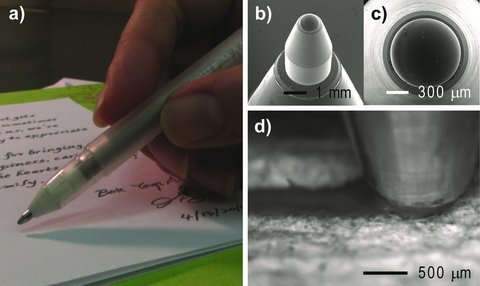
\includegraphics{images/IS_pen-on-paper.jpg}
   \caption{Pen-on-Paper Flexible Electronics. a) Optical image of a rollerball pen loaded with conductive silver ink. b) and c) side and top views of the rollerball pen. d) Optical image of the rollerball pen tip writing a conductive silver track}
   \label{fig:IS_pen-on-paper}
\end{marginfigure}

Inkjet printing allows to pattern of organic semiconductors \cite{kim2008heterogeneous}, metal contacts on organic semiconductors \cite{khan2019soft} \cite{wessely2020sprayable}, and metallic structures that require minimal further processing. Researchers such as Ahn et al. used conductive ink printing to realize metallic connections between functional components of flexible devices.

Another project like that of Russo et al. \cite{russo2011pen} has resulted in an optical image of a flexible paper display containing a LED array \ref{Pen-on-paper}. The prototype is a multi-color 25 × 16 LED array connected to the printed silver electrodes by depositing a drop of concentrated silver ink.

\section{General Architecture}

This project was published and demonstrated at the International Conference on New Interfaces for Musical Expression (NIME) in June 2022. NIME is a research field and conference series that explores innovative ways of creating, performing, and experiencing music through technology and interactive interfaces. It brings together experts from various disciplines such as music, engineering, design, and computer science. 

\subsection{Overview}

Our design augments a traditional paper score in many digital music learning applications on screen-based devices. Children already spend a considerable amount of time in front of screens, which can harm their eyes from a young age. Paper is flexible, lightweight, and easily transportable, and incorporating electronic circuits in the paper has shown its attractiveness to children \cite{hershman2018light}. 

\begin{figure}[h]
   \centering
   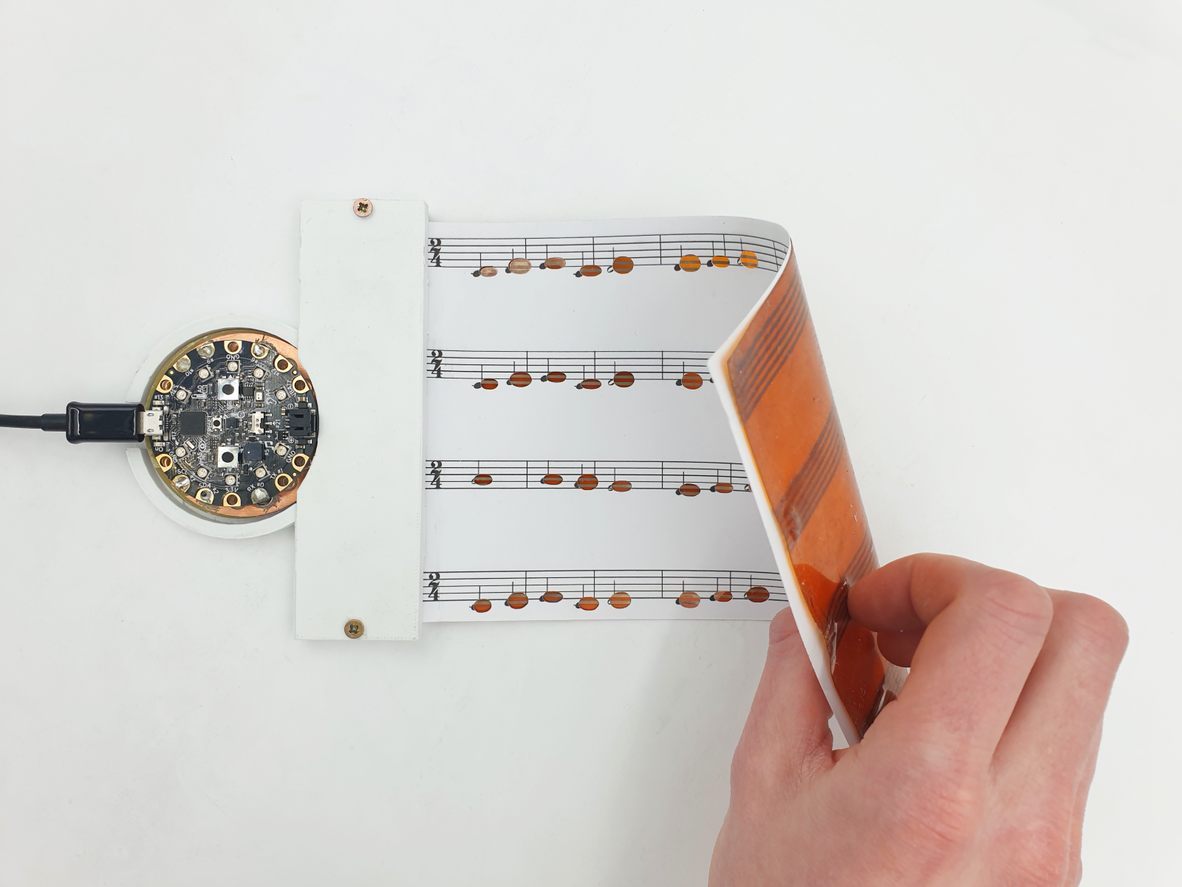
\includegraphics{images/IS_demo.png}
   \caption{Interactive Score Prototype}
   \label{fig:IS_demo}
\end{figure}

The project does not aim to teach a user how to play music. It seeks to link music theory directly with music practice without requiring knowledge.

The user has to supply the electronic part (substrate and PCB), then he places a partition (a cardboard stencil) on top of the substrate (where
the conductive lines are located) \ref{fig:IS_demo}. He can play the music and change it to another one.

\subsection{System Design}

The Interactive score consists of two thin layers. The first layer is the traditional sheet
music, printed on cardstock paper, with holes punched for each note. Under this sheet
is a polyimide substrate with conductive lines printed on it \ref{fig:IS_schema}.

\begin{figure}[h]
   \centering
   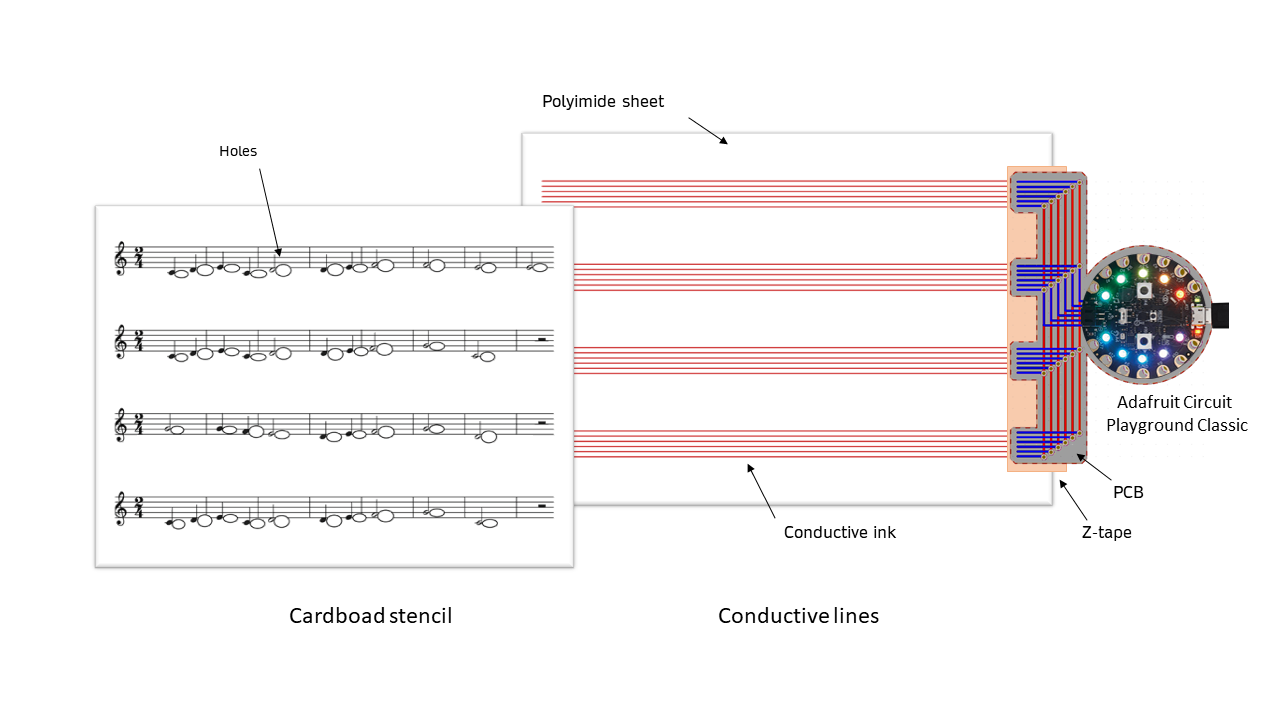
\includegraphics{images/IS_schema.png}
   \caption{Interactive Musical Score architecture.}
   \label{fig:IS_schema}
\end{figure}

The conductive lines are connected to an Adafruit Circuit Playground printed circuit board (PCB) using a double-sided "z-tape".

When the user touches a note on the top layer, the finger makes contact with the conductive lines through the holes in the cardstock.
The signal travels through the ink paths and the z-tape to the PCB, which detects a potential difference using capacitive touch and plays the relevant note. Detecting several simultaneous signals on multiple pins allows playing eleven different notes with only six lines \ref{fig:IS_schema}.

The system is kept in a 3D printed case, maintaining contact between the polyimide, the z tape, and the PCB. The user can easily open and close the case to change the music.



\subsection{Electronic Music Box}

The signal is recovered and used in capacitive touch with an Adafruit Circuit Playground Classic \ref{fig:circuit_playground_classic}. An Arduino program allows for generating a vast number of different notes. The code is retrievable on GitHub \cite{adrien2022capacitive_to_notes}.

\begin{marginfigure}
   \centering
   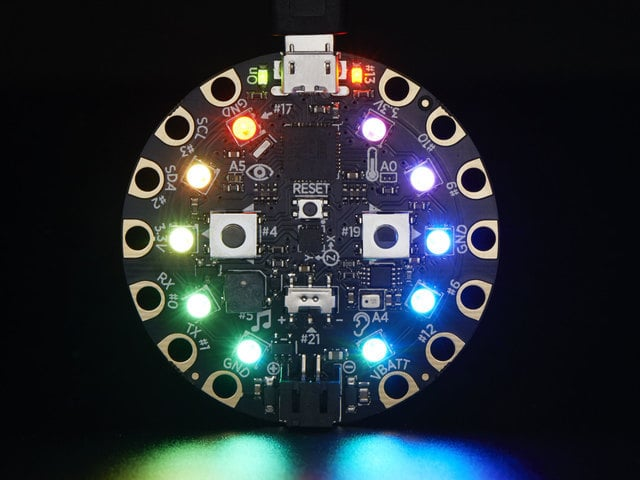
\includegraphics{images/circuit_playground_classic.jpg}
   \caption{Adafruit Circuit Playground Classic}
   \label{fig:circuit_playground_classic}
\end{marginfigure}

About the sound, the Adafruit Circuit Playground embarks a built-in buzzer. The implemented Mini Speaker is the SQMS5002S4036A. This device is a miniature magnetic speaker not adapted for playing detailed audio but for beeping, buzzing, and simple bleepy tunes. It is also possible to change the tone by changing the name of a variable in the code on the microcontroller.

The Adafruit circuit playground has ten mini NeoPixels of all colors, which can be animated with light when a user plays a note. The controller includes motion, temperature, light, sound sensors, a switch, and a mini speaker. This device is ideally suited for use on the score and integrates many features.

\subsection{Paper Score Manufacturing}

Notes, staves, lines, hyphenation, and cutouts were all placed on the same project for perfect dimensional compatibility between the different elements of the score. It allows the elements to fit together perfectly and export the cutout locations at the correct size relative to the partition's rest.

An inkjet printer draws all cardboard lines, hyphens, notes, and numbers.

A score of "J'ai du bon tabac" (on the left) lies on the substrate. Then, the notes were isolated in another PNG file, selected on Cricut design, and cut directly into the cardboard with Cricut maker 3.

% TODO Justifier les choix techniques

\subsection{Conductive Sheet Manufacturing}

The conductive ink paths are 1mm thick and 5cm long, with a resistance of 0.07 Ohms. A simple inkjet printer equipped to print with silver nanoparticles conductive ink drew the lines directly on the substrate. A hoven sintered the printed patterns at 180°C for 73 minutes. This process allows the quick production of flexible circuits \cite{khan2019soft}.

\begin{figure}[h]
   \centering
   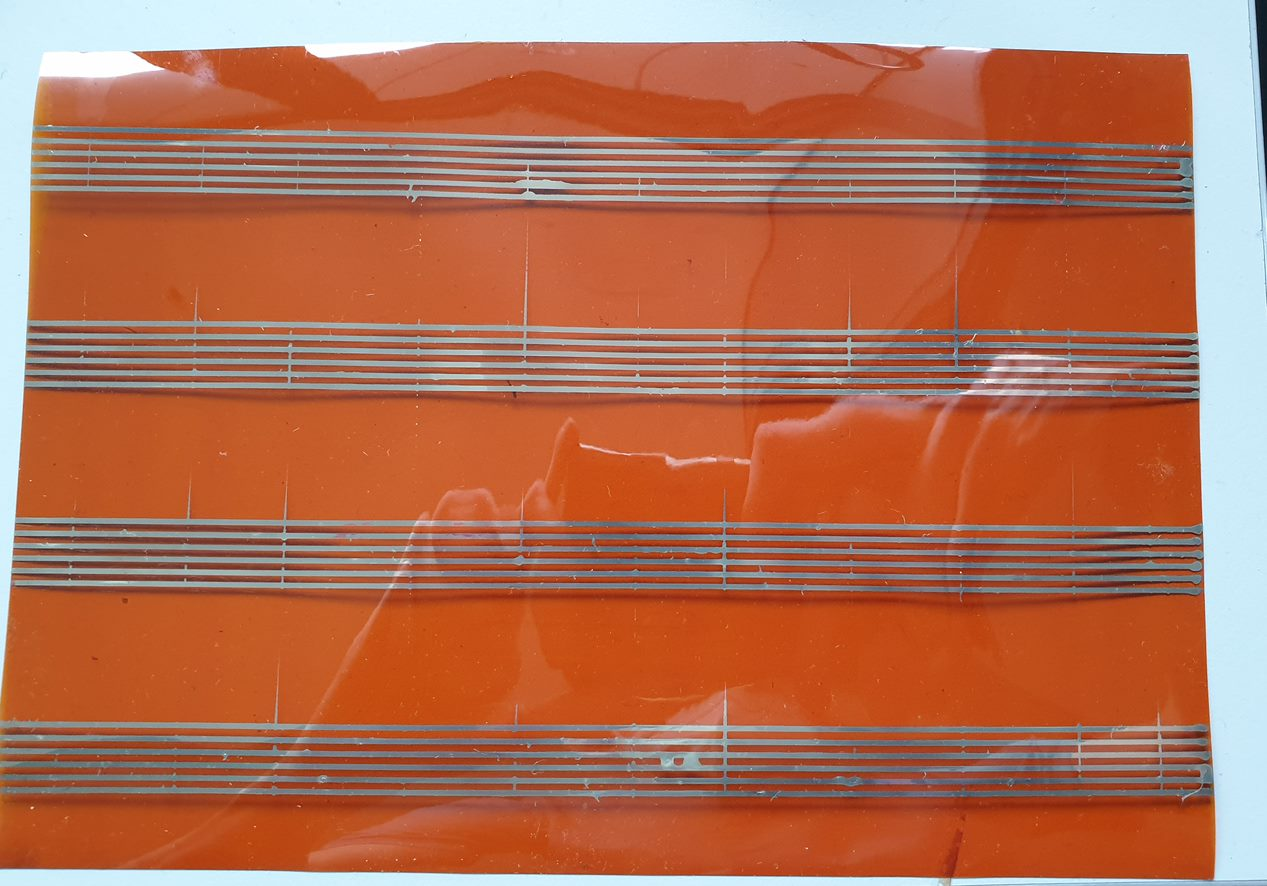
\includegraphics{images/IS_conductive_sheet.jpeg}
   \caption{Interactive Score Conductive Sheet}
   \label{fig:IS_conductive_sheet}
\end{figure}

This prototype comprises four staffs of 6 lines made of conductive ink on a Kapton polyimide sheet substrate. This polymer does not melt at high temperatures and has excellent mechanical strength, and is very dimensionally stable and creep resistant at temperatures above 260°C. The lines are 1mm thick, and at a distance of 15cm in length, it gave a resistance of 0.07 Ohms.

An Epson WF-2010 printer printed the lines on the substrate \cite{adrien2022capacitive_to_notes}.

Conductive ink allows the score to be flexible, like an actual musical score. The use of ink rather than flexible brass strips has the advantage of quickly printing interactive scores on an industrial scale. The material needed is only simple printers and ink and cleaning products for the printers. This process facilitates and accelerates production possibilities.

\subsection{Integration and Usability}

\subsubsection{Ability to change the score}

Its ease of interchangeability and production characterizes the paper score. The user can easily remove the paper sheet from the box and place another to play a different melody. All the electronic parts (substrate, PCB, microcontroller) are independent of the paper score. The sheet music has the exact dimensions of the substrate.
Therefore, placing the two precisely on each other to align the holes with the ink lines is simple.

\subsubsection{Ability to improvise}

The user can improvise by not playing the notes in the same order.
The project allows a great deal of modularity in its use. Just by touching specific notes at certain times, users can experiment with different rhythms and melodies and reconstruct a piece from a few notes.
With a simple score, including an ascending scale, he can try his hand at composition.
It is impossible to create dissonance as the Circuit Playground plays melodies in a fixed tonality set in the code. Unfortunately, this fact also limits the improvisation capacity.


\section{Applications and Evaluation}

\subsection{Set up}

Four users interact with the prototype already prepared for use. They then answer several questions. The project is plugged in and set up as a base for further use. Therefore, measuring the openness and visualization of music theory given by the project to the user is interesting. The questions concern understanding use, practicality, interest, innovation, attractiveness, and playfulness.

\subsection{Results}

The users did not encounter any particular problems during the test. The prototype worked well. The testers gave interesting feedback. The majority of the comments were positive, as the project considered most of their comments since a previous test.

The users proposed many ideas to make the project evolve. They advised adding indications, potentially with LEDs, to indicate actions to be carried out. One idea was to create a binder with different stencils inside. They would have appreciated a correction of the electronics, which would warn them if they made a mistake. The testers liked that the person playing has to press the right notes, unlike some music toys that automatically correct the sound to play the right notes wherever the user presses. The users were also very interested in the fact that the project is portable. They would have liked to be able to take it with them to play music everywhere.

\section{Discussion}

\subsection{Attractivity}

The project could be attractive for children as a tangible object.
Its gamified aspect makes it close to a toy. This aspect contributes to its attractiveness, especially to young children. Its musical property favors the user's creativity in addition to being portable, tactile, fun, and easy to use.

\subsection{Musical Imagery learning}

An essential aspect of musical practice is the ability of the musician to decipher a score. When this one practices with visual support, his brain must take the exercise to connect the note, which he links visually with the position of his fingers on the instrument. The transcription of the note read is an intermediate the brain uses, deducing a position and calculating an interval from it. The ability to translate a visual note into a sound is a reflex to be trained and very relevant in the practice of music. The basics of this ability must be acquired very quickly when learning the basics of music.

\subsection{Mobilizing multiple types of attention}

This kind of device has a genuine interest in terms of learning. The user practices bodily intelligence with touch, visual intelligence since he has a support in front of him, and musical-rhythmic intelligence.

\section{Conclusion}

In conclusion, the interactive score project has a bright future, as it implements a very recent technology to popularize it. This process could be industrialized and even replicable for individuals with some improvements and optimizations. In the future, our goal is to make the score more accessible. Features such as flexibility and a simple "plug and play" aspect make it attractive even to children.

\subsection{Limitations}

The project has some limitations being a prototype. The device is limited in terms of the number of playable notes. The conductive sheet has six lines of conductive ink, which allows for playing 13 different notes between C5 and F6. It is not possible to generate alterations while playing. This fact means that if the playground circuit is set in a specific key, it is impossible to play a note with an alteration not present in the score's framework. The key must also be changed manually at each score change (paper sheet).

The major problem of the prototype is in its transmission of electrical signals.
The most crucial problem of the project is its sensitivity to the electric field due to the use of capacitive touch. Near electric fields, the microcontroller can detect false contacts. The device must also be connected to a power outlet so that the potential difference calculated between the user's finger and the ground is remarkable. Otherwise, the playground circuit may not detect the touch of a line or start playing by itself because of the detection of surrounding electric fields. A user should therefore keep the device at a distance from electronic devices and metal surfaces.

Z-tape transmits the signal from the conductive sheet to the PCB (inside the box). This conductive tape can be damaged and cause false contacts after many uses and transport. The tape can not transmit the current to the lines, and some notes stop working.

Another problem is the conductive ink which can crumble, preventing the current from crossing certain lines. The ink traces are indeed quite fragile and easily damaged. The ink is only dried on the substrate, so its adhesion can weaken. As the user has to run his finger over the ink, he can also remove thin layers, thus causing some lines to break.

The prototype also presents a difficulty in overlaying the sheet paper on top of the polyimide sheet to align the notes with the ink lines while keeping a flexible system. The case was designed for this purpose but could be more effective.

The device also needs to be improved in terms of sound quality.
The speaker driver circuitry is an on/off transistor, so the device can only play square waves. The device's loudest frequency is around 4 KHz. The sound generated is shrill, very electronic, and of poor quality. It can thus slow down the desire to practice and does not resemble the sound of an instrument.

\subsection{Future works}

Adding the play of an alteration with three "buttons" usable thanks to the capacitive touch: flat, sharp, and natural, which the user can trigger with the index finger of the left hand, is an idea to answer the problem of changing the key. These buttons will allow the user to discover the notion of these three tools and their meaning. They would be an interesting tool that would add an improvisation capacity to the system.

A "musical tutorial" should be added so the user can listen to the score's music before playing it. The tutorial would allow the user to assimilate the musical rhythm (the time between playing each note) with the physical rhythm (the time between pressing notes).

The electronic PCB/microcontroller part should also be redesigned to no longer integrate an Adafruit Circuit Playground but a much smaller, handmade circuit. It would be possible to improve the speaker's quality and connect the device to Bluetooth or Wi-Fi to play music at a distance.
The next steps are also about looking for partnerships in children's education to research experimentations on the impact of this interactive score on music assimilation. Several parameters would be evaluated, such as concentration level, playing time, and knowledge retention. It is necessary to consider different strategies to transcript musical-rhythmic on this interactive score.
